\documentclass[12pt]{article}
\usepackage{amssymb,amsmath,latexsym,amsthm,graphicx,url,caption,subcaption,verbatim}
\begin{document}
\title{CS 698R Final Project Report}
\author{Matthew Webb, Abraham Frandsen}
\date{11 December 2014}

\maketitle

\subsection*{Introduction}
Over the course of the semester, we had the opportunity not only to learn about
Bayesian Networks in class, but also to learn about undirected graphical models under
the tutelage of Dr. Ringger. We therefore determined to use techniques from both
areas in this project.
We chose to engage the task of image segmentation due to our joint interest in the problem
as well as to apply our modeling techniques to a realm outside of natural language processing.

We designed and implemented a probabilistic graphical model for image segmentation, together
with a learning algorithm for the model.
Our model consists of both directed and undirected elements.
We used a Gibbs sampling approach for parameter learning, and performed experiments on several
test images.

\subsection*{The Model}
\begin{figure}
\begin{align*}
&N, M \qquad &&\text{Dimensions of image (rows, columns).}\\
&d \qquad &&\text{Dimension of color space.}\\
&K \qquad &&\text{Number of segments/clusters.}\\
&X_{i,j}, \,\, 1\leq i \leq N, 1\leq j \leq M &&\text{Observed value for $(i,j)$-th pixel.}\\
&Z_{i,j}, \,\, 1\leq i \leq N, 1\leq j \leq M &&\text{Cluster assignment for $(i,j)$-th pixel.}\\
&\theta_k,\,\, 1\leq k \leq K &&\text{Parameter vector for cluster $k$.}\\
&X = (X_{i,j})_{1\leq i \leq N, 1 \leq j \leq M}\\
&Z = (Z_{i,j})_{1\leq i \leq N, 1 \leq j \leq M}\\
&\theta = (\theta_k)_{1\leq k \leq K}
\end{align*}
\caption{Basic notation.}
\label{equations}
\end{figure}
See Figure \ref{equations} for the basic notational definitions.
We use the terms cluster and segment interchangeably.
We note that each pixel value $X_{i,j}$ belongs to $\mathbb{R}^d$
(for example, $d=3$ in the case of an RGB image, and $d=1$ in the case
of a grayscale image), and that each $Z_{i,j}$ belongs to the set
$\{1,2,\ldots,K\}$.
Each cluster $k$ has a corresponding probability distribution over pixel values
with parameters $\theta_k$. Depending on the choice of distribution,
$\theta_k$ may be a tuple of one or multiple values.
We call $X$ the pixel emissions, $Z$ the cluster assignments for the image, and
we refer to $\theta$ as the pixel emission parameters.

We designed a hybrid directed-undirected graphical joint probability model over $X, Z$, and $\theta$.
On a high level, our model factorizes as follows:
\[
P(X,Z,\theta) = P(Z)\left(\prod_{k=1}^KP(\theta_k)\right)
\left(\prod_{i=1}^N\prod_{j=1}^MP(X_{i,j}\,|\theta_{Z_{i,j}})\right)
\]
In the generative story,
first draw the cluster assignments $Z$ from the cluster assignment distribution $P(Z)$.
Next, for each cluster $k$, draw the pixel emission parameters $\theta_k$ from $P(\theta_k)$.
Finally, for each pixel $(i,j)$, generate the pixel emission value $X_{i,j}$ given its
cluster assignment $Z_{i,j}$ and the pixel emission parameters $\theta$.

We note that in this model, each pixel emission variable $X_{i,j}$ is conditionally
independent of all other
variables given its cluster assignment $Z_{i,j}$ and the parameters $\theta_{Z_{i,j}}$
corresponding to the cluster assignment. Further, each $\theta_k$ is independent of all
other $\theta_l$, for $l \neq k$. These independence properties are reflected
directly in the factorization of the joint probability.

We model the relationships between the cluster assignment variables $Z_{i,j}$ with an undirected graph
$\mathcal{G}$ over these variables.
In particular, for $1 \leq i \leq N$ and $1 \leq j \leq M$, let
\[
D_{i,j} = \{Z_{i+\epsilon_1,j+\epsilon_2}\,|\,-1 \leq \epsilon_1, \epsilon_2 \leq 1\},
\]
i.e. $D_{i,j}$ is the $3\times 3$ subgrid of cluster assignment variables centered at $Z_{i,j}$
(with obvious adjustments made for the edges of the image). Let each $D_{i,j}$ be a clique in
$\mathcal{G}$, and for each clique $D_{i,j}$, define a clique potential $\phi_{i,j}(D_{i,j})$
(a real-valued function).
Let $\mathcal{C}$ denote the collection of cliques $D_{i,j}$.
This gives a Markov random field over $Z$ of the form
\[
P(Z) = \frac{1}{\mathcal{Z}}\prod_{i=1}^N\prod_{j=1}^M \phi_{i,j}(D_{i,j}),
\]
where $\mathcal{Z}$ is the partition function.
Since each clique $D_{i,j}$ is of the same form as all others,
it is reasonable to set all clique potentials equal to the same function.
Thus, to fully specify the distribution $P(Z)$, we need only define one clique potential $\phi$.
We discuss our choice of $\phi$ later in this report. Figure \ref{fig:graph} gives a graphical
depiction of the key elements of the model.

\begin{figure}
    \begin{center}
        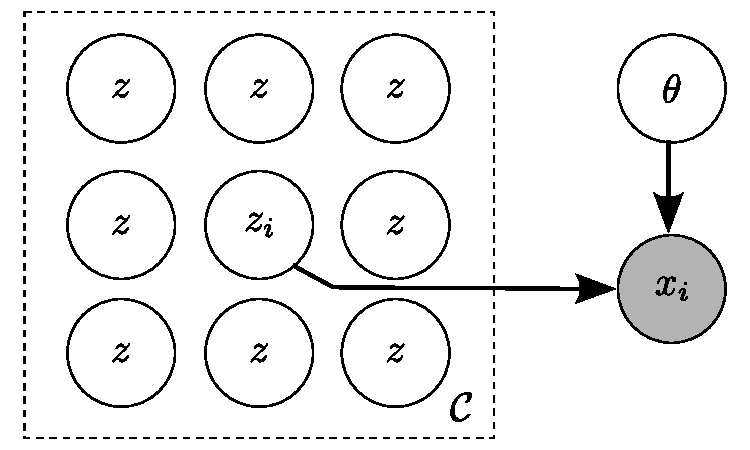
\includegraphics[height=2in]{graph.pdf}
        \caption{Graphical representation of atomic model component}
        \label{fig:graph}
    \end{center}
\end{figure}

We opt for a MCMC approach to learning the cluster assignments and pixel emission parameters.
In particular, given an image (i.e. given the pixel emissions $X$), we use Gibbs sampling
to generate draws from $P(Z,\theta\, |\, X)$.
Deriving the complete conditionals for each $\theta_k$ and $Z_{i,j}$ is straightforward,
and we detail them later in the report.

\subsection*{Data}
We use our model with two different images. The first is a cropped photo of a
rock formation in Monument Valley. The original photo is attributed to a user
named Huebi and is taken from Wikipedia. Further details can be found at
\url{http://en.wikipedia.org/wiki/Monument_Valley#mediaviewer/File:Monument_Valley_2.jpg}.
This image has a distinct skyline against a fairly homogenous rock formation.
The second image is property of one of the authors. It is a more complex image
of a baby girl, and has more subtle changes in tone and texture throughout.
Both images were cropped to a very small size to permit quick computation.

\begin{figure}
    \begin{center}
        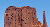
\includegraphics[width=2in]{small/mv_small.png}
    \end{center}
    \caption{Photo of Monument Valley}
\end{figure}

\begin{figure}
    \begin{center}
        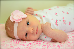
\includegraphics[width=2in]{small/esther_small.png}
    \end{center}
    \caption{Photo of baby girl}
\end{figure}

\subsection*{Design Decisions}
We chose the pixel emission distribution for each cluster to be a multivariate normal
distribution parameterized by a mean vector and precision matrix.
Thus, for each $k$ we have $\theta_k = (\mu_k, \Lambda_k)$ (mean vector and precision matrix,
respectively), and for each pixel $(i,j)$
we have
\[
X_{i,j} \sim MVN(\mu_{Z_{i,j}}, \Lambda_{Z_{i,j}}).
\]
For each cluster $k$, we let $\mu_k$ and $\Lambda_k$ be independent according
to the prior distribution $P(\theta_k)$, so that
\[
P(\theta_k) = P(\mu_k)P(\Lambda_k).
\]
We assumed a multivariate normal distribution for each $\mu_k$ and a
$d$-dimensional Wishart distribution for each $\Lambda_k$, i.e.
\begin{align*}
\mu_k &\sim MVN(m,S), \qquad && k=1,2,\ldots,K\\
\Lambda_k &\sim W_d(V,n), &&k=1,2,\ldots,K,
\end{align*}
where
\begin{align*}
n &= 4\\
m &= \begin{bmatrix}
0 & 0 & 0
\end{bmatrix}^T\\
V &= \begin{bmatrix}
1 & 0 & 0\\
0 & 1 & 0\\
0 & 0 & 1
\end{bmatrix}\\
S &= .0001\begin{bmatrix}
1 & 0 & 0\\
0 & 1 & 0\\
0 & 0 & 1
\end{bmatrix}.
\end{align*}
These distributions are conjugate to the multivariate normal distribution, and hence allow for
efficient sampling from the complete conditionals in the Gibbs sampler. The hyperparameters
were chosen to make these priors relatively uninformative.
In practice, we shift the image by its mean before running the sampler,
which justifies our choice for the hyperparameter $m$.

Under these conjugate prior distributions, the complete conditionals for $\mu_k$ and $\Lambda_k$
are again multivariate normal and Wishart, respectively.
The complete conditional for each $Z_{i,j}$ is simply a categorical distribution with weight
vector $\omega$. This weight vector is found by first calculating each component
\[
\omega_k = P(X_{i,j}\,|\,\theta_k)
\prod_{\substack{D \in \mathcal{C}\\
        Z_{i,j} \in D}}\phi(D), \quad \text{(where we set $Z_{i,j}=k$)}
\]
and then normalizing so that it sums to 1.

\begin{table}
    \begin{center}
    \begin{tabular}{| l | l |}
        \hline
        shape & weight \\ \hline
        
\includegraphics[width=5mm]{shapes/255.png} & 3\\
        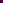
\includegraphics[width=5mm]{shapes/31.png} & 2\\
        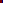
\includegraphics[width=5mm]{shapes/107.png} & 2\\
        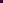
\includegraphics[width=5mm]{shapes/11.png} & 1\\
        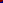
\includegraphics[width=5mm]{shapes/15.png} & 1\\
        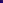
\includegraphics[width=5mm]{shapes/22.png} & 1\\
        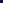
\includegraphics[width=5mm]{shapes/1.png} & -1\\
        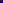
\includegraphics[width=5mm]{shapes/19.png} & -1\\
        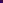
\includegraphics[width=5mm]{shapes/209.png} & -1\\
        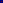
\includegraphics[width=5mm]{shapes/0.png} & -2\\
        \hline
    \end{tabular}
    \end{center}
    \caption{Weights for selected shapes.}
    \label{table:shapes}
\end{table}

The choice of weights for the clique potentials is the fundamental way in which
we incorporate our prior belief about the arrangement of image segments,
especially since we are not learning these weights from labelled data. We adopt
an intuitive approach to choosing these weights. We wish to assert local shapes
that we would imagine could be a part of an image segment, and penalize those
shapes that we do not think are so. Since we are looking at the comparison of
the eight labels that surround the center label, there are $2^8 = 256$ possible
shapes. When we consider rotations of the same shape to be equivalent, this
number becomes even more manageable.

We chose to assign a beneficial weight to a subset of the shapes and their
rotations. We assign the most favorable weight to the shape in which all labels
are equal. We assign somewhat favorable weights to the shapes which could be
part of an edge, that is, which partition the labels into two connected
segments not including diagonals. All other shapes are assigned a penalizing
weight. Some examples are given in Table \ref{table:shapes}.

This choice of prior is similar to the Ising model. In the Ising model, all
cliques are pairs of neighbors. This structure is able to assert that neighbors
should mostly be the same label. However, it is not able to assert the likely
boundaries between two segments. Our generalization hopes to assert likely
boundaries along with the core idea that neighbors should mostly be the same
label.

\subsection*{Results}

\begin{figure}
    \begin{center}
        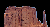
\includegraphics[width=2in]{results/mv_1.png}
    \end{center}
    \caption{Segmented Monument Valley}
    \label{fig:mv}
\end{figure}

\begin{figure}
        \centering
        \begin{subfigure}[b]{0.3\textwidth}
                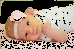
\includegraphics[width=\textwidth]{results/esther_0_1.png}
                \caption{No prior}
                \label{fig:esther_0}
        \end{subfigure}%
        ~ %add desired spacing between images, e. g. ~, \quad, \qquad, \hfill etc.
          %(or a blank line to force the subfigure onto a new line)
        \begin{subfigure}[b]{0.3\textwidth}
                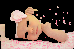
\includegraphics[width=\textwidth]{results/esther_3_0.png}
                \caption{With prior}
                \label{fig:esther_1}
        \end{subfigure}
        ~ %add desired spacing between images, e. g. ~, \quad, \qquad, \hfill etc.
          %(or a blank line to force the subfigure onto a new line)
        %\begin{subfigure}[b]{0.3\textwidth}
        %        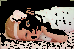
\includegraphics[width=\textwidth]{results/esther_1_0.png}
        %        \caption{With prior}
        %        \label{fig:esther_2}
        %\end{subfigure}
        \caption{Segments with and without prior}\label{fig:esthers}
\end{figure}

The image from Monument Valley (see Figure \ref{fig:mv}) was segmented in the
same way both using a prior and without using a prior on segments. The colors
were fairly homogenous in both visually apparent segments, and the segments
found by the algorithm agree with intuition.

The image of the baby girl (see Figure \ref{fig:esthers}) presents a more
interesting case. There are a number of different textures and colors, and it
is not obvious what the two segments should be. The model that had no prior on
segments identified the back wall, but also plucked out the pink highlights in
the foreground. When a prior was included, the model was able to overcome this
issue somewhat. Though there is still some scattered pink highlights, it is not
as extreme as the first case.


\subsection*{Qualitative Evaluation}
Our choice to model the pixel emissions for each cluster as a multivariate normal has important
implications on the quality of the segments that we obtain.
Essentially, this modeling choice assumes that each segment in the image is characterized by just one
color value, and that each pixel emission in the segment should be close to this characteristic
color. This suggests that the model will struggle with finding segments that are characterized
not by a dominant color, but by distinctive textures or contrast. 
An example of this is shown in Figure \ref{fig:esther_1}, where the segment containing the background
and the baby's shirt leaves out the pink-colored pixels, even though to the human eye, they should be
lumped together in that same segment.
Perhaps one way to improve the model in this respect would be to make each
pixel emission distribution a mixture of multivariate normals, allowing for varying colors to feature
prominently in the segments.

Another salient point related to the pixel emissions is the choice of color space used to represent
the image.
In our experiments, we used the standard RGB color channels to represent each pixel emission.
However, this color space may not always correspond closely with human perception of which colors are
close or far apart.
Thus, two pixels that a human eye might judge to be similar in color may be assigned to different
segments, simply because the actual RGB values are far apart.
Choosing a color space that most closely matches how the human eye perceives and judges color may
lead to better performance, although we are unaware of whether such an ideal color space exists.

We hope that the decisions made about the prior structure of the segments will
help the model be less sensitive to pixel anomalies that might be present if
the labels were treated as independent. For example, if a single pixel was a
different color than most of its neighbors, the prior influence would hopefully
be such that this anomaly would be ``squeezed out'', and it would be labelled
with its neighbors.

There is a trade-off between the size of the cliques and the complexity of their
implementation and computation. Since we are not learning the factor weights,
but rather specifying them ``by hand'', more complex cliques would result in
more time spent making decisions about which shapes to assert or penalize.
Also, every clique of which an individual label is a member needs to be
including in the Gibbs sampling update. So the computational complexity
increasing with the complexity of the cliques.

Since we choose to work with small, simple cliques, their influence is mostly
seen at the local level. They are able to help influence the micro-structures
that are exhibited among the segments. However, they do not have a macroscopic
view of the problem. This can result in fragmented segments.

\subsection*{Conclusion}
This model presents interesting ideas about image segmentation, and also
demonstrates important shortcomings. The structure for the prior distribution
of segments allows an interesting paradigm in which to work. However, there are
certain deficiencies that necessarily arise when working on a local scale.

One important decision we made as modelers was to use a generative model. This
gave us an intuitive way to approach the problem. However, we feel like it
would be worthwhile to explore using conditional models for this problem.
Generating new images with the model does not have many apparently practical
purposes. Using a generative model would allow the distribution on a label to
involve not only the pixel emission it labels, but also the emissions of its
neighbors or others. This would allow another mechanism to help detect
boundaries.

By completing this project, we learned a lot about specifying and working with
hybrid directed-undirected graphical models. Also, we developed our intuition
about what important questions need to be answered when segmenting an image.
Finally, we developed our modeling abilities by creating and working with a new
probability model.

\subsection{Selected Code}

\begin{verbatim}

# Authors: Matthew Webb, Abe Frandsen
import sys

from utils import wishart, logNormPDF, logWisPDF, inv3
from factors import phi
from phi import phi_all, phi_blanket

from numpy import zeros, ones, log, exp, sum, mean, dot, array, eye, outer
from numpy import allclose, load, abs, max
from numpy.random import randint, random, multivariate_normal as mvn
from scipy.stats.distributions import norm, gamma
from scipy.misc import logsumexp

from utils import wishart, logNormPDF, logWisPDF, inv3
from phi import phi_all, phi_blanket
from numpy import load

FS = load('factors.npy') # allow optimized computation

def segment(image, n_segments=2, burn_in=1000, samples=1000, lag=5):
    """
    Return image segment samples.

    Parameters
    ----------
    image : (N,M,3) ndarray
        Pixel array with 3-dimensional values (e.g. RGB)

    Returns
    -------
    labels : (samples,N,M) ndarray
        The image segment label array
    emission_mus: (samples,n_segments,3) ndarray
        The Gaussian emission distribution (mean).
    emission_precs : (samples,n_segments,3,3) ndarray
        The Gaussian emission distribution (precision).
    log_prob_p : (samples,) ndarray
        Log probability portion contributed by prior
    log_prob_e : (samples,) ndarray
        Log probability portion contributed by emissions
    """
    N,M = image.shape[:2]
    image = normalize(image)

    # allocate arrays
    res_labels = zeros((samples+1,N,M))
    res_emission_mu = zeros((samples,n_segments,3))
    res_emission_prec = zeros((samples,n_segments,3,3))
    res_log_prob_p = zeros((samples,))
    res_log_prob_e = zeros((samples,))

    # initialize hyperparmeters
    nu = 4 # df hyperparameter for wishart
    V = eye(3) # scale matrix hyperparameter for wishart
    Vinv = inv3(V)
    mu = zeros(3) # mean hyperparameter for MVN
    S = eye(3)*0.0001 # precision hyperparameter for MVN


    # initialize labels/params
    padded_labels = ones((N+2,M+2), dtype=int)*-1
    padded_labels[1:-1,1:-1] = randint(n_segments,size=(N,M))
    labels = padded_labels[1:-1, 1:-1]
    for n in xrange(N):
        for m in xrange(M):
            labels[n,m] = (n*M + m)%n_segments
    res_labels[-1] = labels

    # draw from prior
    emission_mu = mvn(mu,S,size=n_segments)
    emission_prec = array([wishart(V,nu) for i in xrange(n_segments)])
    log_prob_p = None
    log_prob_e = None

    conditional = zeros((n_segments,))

    # gibbs
    for i in xrange(burn_in + samples*lag - (lag - 1)):
        for n in xrange(N):
            for m in xrange(M):
                # resample label
                for k in xrange(n_segments):
                    labels[n,m] = k
                    conditional[k] = 0.
                    conditional[k] += phi_blanket(
                            memoryview(padded_labels), n, m,
                            memoryview(FS))
                    conditional[k] += logNormPDF(image[n,m,:],
                            emission_mu[k], emission_prec[k])
                labels[n,m] = sample_categorical(conditional)

        for k in xrange(n_segments):
            mask = (labels == k)
            n_k = sum(mask)

            # resample label mean
            if n_k:
                P = inv3(S+n_k*emission_prec[k])
                xbar = mean(image[mask],axis=0)
                emission_mu[k,:] = mvn(dot(P,n_k*dot(emission_prec[k],xbar)),P)
            else:
                emission_mu = mvn(mu,S,size=n_segments) # draw from prior

            # resample label precision
            if n_k:
                D = outer(image[mask][0,:]-emission_mu[k,:],
                        image[mask][0,:]-emission_mu[k,:])
                for ii in xrange(1,n_k):
                    D += outer(image[mask][ii,:]-emission_mu[k,:],
                            image[mask][ii,:]-emission_mu[k,:])
                emission_prec[k,:,:] = wishart(inv3(Vinv+D),nu+n_k)
            else:
                emission_prec[k,:,:] = wishart(V,nu) # resample using the prior

        log_prob_p = 0.
        log_prob_e = 0.
        for c in xrange(n_segments):
            log_prob_e += logNormPDF(emission_mu[c],mu,S)
            log_prob_e += logWisPDF(emission_prec[c],nu,Vinv)
        for n in xrange(N):
            for m in xrange(M):
                label = labels[n,m]
                log_prob_e += logNormPDF(image[n,m,:],
                        emission_mu[label],emission_prec[label])

        log_prob_p = phi_all(memoryview(padded_labels), memoryview(FS))

        sys.stdout.write('\riter {} prior {} emission {}'.format(i, log_prob_p,
                log_prob_e, sum(labels==0), sum(labels==1)))
        sys.stdout.flush()

        if not sum(labels==0) or not sum(labels==1):
            RETURN_MINUS_ONE = True
            raise ValueError("converged to 0...")

        if i < burn_in:
            pass
        elif not (i - burn_in)%lag:
            res_i = i/lag
            res_emission_mu[res_i] = emission_mu[:,:]
            res_emission_prec[res_i] = emission_prec[:,:,:]
            res_labels[res_i] = labels
            res_log_prob_p[i] = log_prob_p
            res_log_prob_e[i] = log_prob_e

    sys.stdout.write('\n')

    return (res_labels, res_emission_mu, res_emission_prec, res_log_prob_p,
            res_log_prob_e)

def normalize(image):
    """Subtract means from image."""
    image = image.copy().astype(float)
    image -= array([image[:,:,i].mean() for i in xrange(3)])
    return image

def sample_categorical(p):
    """Sample a categorical parameterized by (unnormalized) exp(p)."""
    q = exp(p - logsumexp(p))
    r = random()
    k = 0
    while k < len(q) - 1 and q[k] <= r:
        r -= q[k]
        k += 1
    return k

--------------------

from numpy import outer, dot, zeros, empty, inner, trace
from numpy.random import multivariate_normal as mvn
from math import sqrt, log

def wishart(sig, n):
    """
    Sample from a Wishart distribution (naive implementation).

    Parameters
    ----------
    sig : (d,d) ndarray
        The scale matrix for the Wishart distribution, must be pos. definite.
    n : int
        Must be >= d.

    Returns
    -------
    w : (d,d) ndarray
        The sample from the distribution.
    """
    d = sig.shape[0]
    X = mvn(zeros(d), sig, n)
    return dot(X.T,X)

def det3(A):
    """Return the determinant of a 3x3 matrix."""
    return (A[0,0]*A[1,1]*A[2,2]+A[0,1]*A[1,2]*A[2,0]+
            A[0,2]*A[1,0]*A[2,1]-(A[0,2]*A[1,1]*A[2,0]+
            A[0,0]*A[1,2]*A[2,1]+A[0,1]*A[1,0]*A[2,2]))

def inv3(A):
    """Return the inverse of a 3x3 matrix."""
    I = empty((3,3))
    I[0,0] = A[1,1]*A[2,2]-A[1,2]*A[2,1]
    I[1,1] = A[0,0]*A[2,2]-A[0,2]*A[2,0]
    I[2,2] = A[0,0]*A[1,1]-A[0,1]*A[1,0]
    I[1,0] = -A[1,0]*A[2,2]+A[1,2]*A[2,0]
    I[0,1] = -A[0,1]*A[2,2]+A[0,2]*A[2,1]
    I[2,0] = A[1,0]*A[2,1]-A[1,1]*A[2,0]
    I[0,2] = A[0,1]*A[1,2]-A[0,2]*A[1,1]
    I[2,1] = -A[0,0]*A[2,1]+A[0,1]*A[2,0]
    I[1,2] = -A[0,0]*A[1,2]+A[0,2]*A[1,0]
    d = det3(A)
    return I/d

def logNormPDF(x,mu,V):
    """
    Return the log of the PDF of a MVN with mean mu and precision V
    evaluated at x (up to additive constant of proportionality).

    Parameters
    ----------
    x : (d,) ndarray
    mu : (d,) ndarray
    V : (d,d) ndarray
        Must be symmetric, positive definite

    Returns
    -------
    d : float
    """
    return sqrt(det3(V))-0.5*inner(x-mu,V.dot(x-mu))

def logWisPDF(X,nu,Vinv):
    """
    Return the log of the PDF of a wishart with parameters nu, V
    evaluated at X (up to additive constant of proportionality not
    dependent on X).

    Parameters
    ----------
    X : (3,3) ndarray
        Must be positive definite.
    nu : int
        Must be >= 3
    Vinv : (3,3) ndarray
        The inverse of the scale matrix V of the distribution

    Returns
    -------
    logpdf : float
    """
    return (nu-4)/2.*log(det3(X)) - .5*log(trace(dot(Vinv,X)))

--------------------

#include "phi.h"

static PyMethodDef phiMethods[] = {
    {"phi", phi, METH_VARARGS, "plabels, n, m, factors"},
    {"phi_blanket", phi_blanket, METH_VARARGS, "plabels, n, m, factors"},
    {"phi_all", phi_all, METH_VARARGS, "plabels, factors"},
    {NULL, NULL, 0, NULL}
};

PyMODINIT_FUNC initphi(void) {
    Py_InitModule("phi", phiMethods);
}

static PyObject *phi(PyObject *self, PyObject *args) {

    Py_buffer b_plabels, b_factors;
    int64_t *plabels;
    int n, m, N, M, phi_key, label, comp;
    double *factors;

    if (!PyArg_ParseTuple(args, "w*iiw*", &b_plabels, &n, &m, &b_factors))
        return NULL;

    // Check plabels
    if (b_plabels.ndim != 2) {
        PyErr_SetString(PyExc_ValueError, "expected 2d plabels");
        return NULL;
    }
    plabels = b_plabels.buf;
    N = b_plabels.shape[0] - 2; // shape of original image
    M = b_plabels.shape[1] - 2; // shape of original image
    if (n < 0 || n > N-1) {
        PyErr_SetString(PyExc_ValueError, "incorrect index n");
        return NULL;
    }
    if (m < 0 || m > M-1) {
        PyErr_SetString(PyExc_ValueError, "incorrect index m");
        return NULL;
    }

    // Check factors
    if (b_factors.ndim != 1 && b_factors.shape[0] != 256) {
        PyErr_SetString(PyExc_ValueError, "expected factors of shape (256,)");
        return NULL;
    }
    factors = b_factors.buf;

   // Compute
    phi_key = 0;
    label = plabels[(n+1)*(M+2) + m+1];
    phi_key += (int)(plabels[(n+0)*(M+2) + m+0] == label) << 0;
    phi_key += (int)(plabels[(n+1)*(M+2) + m+0] == label) << 1;
    phi_key += (int)(plabels[(n+2)*(M+2) + m+0] == label) << 2;
    phi_key += (int)(plabels[(n+0)*(M+2) + m+1] == label) << 3;
    phi_key += (int)(plabels[(n+2)*(M+2) + m+1] == label) << 4;
    phi_key += (int)(plabels[(n+0)*(M+2) + m+2] == label) << 5;
    phi_key += (int)(plabels[(n+1)*(M+2) + m+2] == label) << 6;
    phi_key += (int)(plabels[(n+2)*(M+2) + m+2] == label) << 7;
    return PyFloat_FromDouble(-1.*factors[phi_key]);
}

static PyObject *phi_blanket(PyObject *self, PyObject *args) {

    Py_buffer b_plabels, b_factors;
    int64_t *plabels;
    int n, m, N, M, phi_key, label, i, j, comp;
    double *factors, result;

    if (!PyArg_ParseTuple(args, "w*iiw*", &b_plabels, &n, &m, &b_factors))
        return NULL;

    // Check plabels
    if (b_plabels.ndim != 2) {
        PyErr_SetString(PyExc_ValueError, "expected 2d plabels");
        return NULL;
    }
    plabels = b_plabels.buf;
    N = b_plabels.shape[0] - 2;
    M = b_plabels.shape[1] - 2;
    if (n < 0 || n > N-1) {
        PyErr_SetString(PyExc_ValueError, "incorrect index n");
        return NULL;
    }
    if (m < 0 || m > M-1) {
        PyErr_SetString(PyExc_ValueError, "incorrect index m");
        return NULL;
    }

    // Check factors
    if (b_factors.ndim != 1 && b_factors.shape[0] != 256) {
        PyErr_SetString(PyExc_ValueError, "expected factors of shape (256,)");
        return NULL;
    }
    factors = b_factors.buf;

    // Compute
    result = 0.;
    for (i=max(n-1, 0); i<min(n+2, N); i++) {
        for (j=max(m-1, 0); j<min(m+2, M); j++) {
            phi_key = 0;
            label = plabels[(i+1)*(M+2) + j+1];
            phi_key += (int)(plabels[(i+0)*(M+2) + j+0] == label) << 0;
            phi_key += (int)(plabels[(i+1)*(M+2) + j+0] == label) << 1;
            phi_key += (int)(plabels[(i+2)*(M+2) + j+0] == label) << 2;
            phi_key += (int)(plabels[(i+0)*(M+2) + j+1] == label) << 3;
            phi_key += (int)(plabels[(i+2)*(M+2) + j+1] == label) << 4;
            phi_key += (int)(plabels[(i+0)*(M+2) + j+2] == label) << 5;
            phi_key += (int)(plabels[(i+1)*(M+2) + j+2] == label) << 6;
            phi_key += (int)(plabels[(i+2)*(M+2) + j+2] == label) << 7;
            result -= factors[phi_key];
        }
    }
    return PyFloat_FromDouble(result);
}

static PyObject *phi_all(PyObject *self, PyObject *args) {

    Py_buffer b_plabels, b_factors;
    int64_t *plabels;
    int N, M, phi_key, label, i, j, comp;
    double *factors, result;

    if (!PyArg_ParseTuple(args, "w*w*", &b_plabels, &b_factors))
        return NULL;

    // Check plabels
    if (b_plabels.ndim != 2) {
        PyErr_SetString(PyExc_ValueError, "expected 2d plabels");
        return NULL;
    }
    plabels = b_plabels.buf;
    N = b_plabels.shape[0] - 2;
    M = b_plabels.shape[1] - 2;

    // Check factors
    if (b_factors.ndim != 1 && b_factors.shape[0] != 256) {
        PyErr_SetString(PyExc_ValueError, "expected factors of shape (256,)");
        return NULL;
    }
    factors = b_factors.buf;

    // Compute
    result = 0.;
    for (i=0; i<N; i++) {
        for (j=0; j<M; j++) {
            phi_key = 0;
            label = plabels[(i+1)*(M+2) + j+1];
            phi_key += (int)(plabels[(i+0)*(M+2) + j+0] == label) << 0;
            phi_key += (int)(plabels[(i+1)*(M+2) + j+0] == label) << 1;
            phi_key += (int)(plabels[(i+2)*(M+2) + j+0] == label) << 2;
            phi_key += (int)(plabels[(i+0)*(M+2) + j+1] == label) << 3;
            phi_key += (int)(plabels[(i+2)*(M+2) + j+1] == label) << 4;
            phi_key += (int)(plabels[(i+0)*(M+2) + j+2] == label) << 5;
            phi_key += (int)(plabels[(i+1)*(M+2) + j+2] == label) << 6;
            phi_key += (int)(plabels[(i+2)*(M+2) + j+2] == label) << 7;
            result -= factors[phi_key];
        }
    }
    return PyFloat_FromDouble(result);
}
\end{verbatim}

\end{document}
